\documentclass[11pt,a4paper]{article}

% =================================================================
%  Question Bank -- Unit I: Basics of Automation and Control
%  Self-contained: all block diagrams / flowcharts drawn with TikZ.
% =================================================================

\usepackage[margin=2cm, headheight=14pt]{geometry}
\usepackage{amsmath}
\usepackage{amssymb}
\usepackage{bm}
\usepackage{array}
\usepackage{booktabs}
\usepackage{enumitem}
\usepackage{xcolor}
\usepackage{tikz}
\usepackage[most]{tcolorbox}
\usepackage{fancyhdr}
\usepackage{helvet}
\renewcommand{\familydefault}{\sfdefault}
\setlength{\emergencystretch}{2em}

\usetikzlibrary{shapes.geometric, arrows.meta, positioning, calc, fit, backgrounds, patterns}

% -------------------------------------------------
% Colour palette (same as the lecture decks)
% -------------------------------------------------
\definecolor{cAccent}{RGB}{0,102,153}
\definecolor{cGreen}{RGB}{34,139,34}
\definecolor{cRed}{RGB}{178,34,34}
\definecolor{cOrange}{RGB}{204,102,0}
\definecolor{cPurple}{RGB}{102,45,145}
\definecolor{cGrayBg}{RGB}{245,246,248}

% -------------------------------------------------
% TikZ styles
% -------------------------------------------------
\tikzset{
	process/.style  ={rectangle, minimum width=2.6cm, minimum height=0.8cm, text centered, align=center, text width=2.6cm, draw=black, fill=blue!8},
	decision/.style ={diamond, aspect=2, minimum width=2.4cm, minimum height=0.9cm, text centered, text width=2.4cm, draw=black, fill=cGreen!18, inner sep=1pt},
	startstop/.style={rectangle, rounded corners=8pt, minimum width=2.2cm, minimum height=0.7cm, text centered, align=center, draw=black, fill=cAccent!25},
	flowarrow/.style={-{Stealth[length=2.5mm]}, thick},
	blk/.style      ={rectangle, draw=black, thick, minimum width=1.9cm, minimum height=0.9cm, align=center, fill=blue!8},
	sumj/.style     ={circle, draw=black, thick, minimum size=0.55cm, inner sep=0pt},
	sig/.style      ={-{Stealth[length=2.2mm]}, thick},
	vflow/.style    ={-{Stealth[length=2mm]}, thick},
}
% valve-symbol helpers
\newcommand{\vspring}[2]{%
	\draw[thick] (#1,#2) -- ++(0.08,0.18) -- ++(0.1,-0.36) -- ++(0.1,0.36) -- ++(0.1,-0.36) -- ++(0.1,0.36) -- ++(0.08,-0.18);}
\newcommand{\vsolenoid}[2]{%
	\draw[thick] ({#1-0.45},{#2-0.22}) rectangle (#1,{#2+0.22});
	\draw[thick] ({#1-0.45},{#2-0.22}) -- (#1,{#2+0.22});}
\newcommand{\vblock}[3]{%
	\draw[thick] (#1,#2) -- (#1,{#2+#3});
	\draw[thick] ({#1-0.12},{#2+#3}) -- ({#1+0.12},{#2+#3});}

% -------------------------------------------------
% Question / answer layout
% -------------------------------------------------
\newcommand{\opts}[4]{%
	\par\smallskip
	\begin{tabular}{@{}p{0.46\linewidth}p{0.46\linewidth}@{}}
		(a) #1 & (b) #2 \\
		(c) #3 & (d) #4 \\
	\end{tabular}\par}
\newcommand{\ans}[1]{%
	\par\smallskip
	{\color{cGreen!50!black}\textbf{Answer:} #1}\par\medskip}
\newtcolorbox{answer}{breakable, enhanced, colback=cGreen!4, colframe=cGreen!55!black,
	boxrule=0.6pt, arc=2pt, left=6pt, right=6pt, top=4pt, bottom=4pt,
	title={Answer}, fonttitle=\bfseries\small, coltitle=white}
\newcommand{\qmarks}[1]{\hfill\textbf{[#1]}}
\newcommand{\partheading}[2]{%
	\bigskip
	\begin{tcolorbox}[colback=cAccent!10, colframe=cAccent, boxrule=0.6pt, arc=2pt, left=6pt, top=3pt, bottom=3pt]
		\textbf{\large #1} \hfill \textbf{#2}
	\end{tcolorbox}}

\setlist[enumerate,1]{label=\textbf{Q\arabic*.}, leftmargin=*, itemsep=6pt}

\pagestyle{fancy}
\fancyhf{}
\lhead{\small Question Bank --- Unit I}
\rhead{\small Basics of Automation and Control}
\cfoot{\small \thepage}

\begin{document}

	% -------------------------------------------------
	% Title block
	% -------------------------------------------------
	\begin{center}
		{\Large\bfseries\color{cAccent} Question Bank}\\[4pt]
		{\large\bfseries Unit I: Basics of Automation and Control}\quad(09 Hrs.)\\[6pt]
		{\small Amit Kumar Singh, Assistant Professor (ECE), School of Naval Architecture and Ocean Engineering\\
			Indian Maritime University, Visakhapatnam Campus}
	\end{center}

	\noindent\textbf{Syllabus:} Brief introduction about industrial processes and their automation; elements of pneumatic, hydraulic and electrical control systems; valves and actuators; stepper motors; PID controllers and their tuning.

	\medskip
	\noindent
	\begin{tabular}{@{}lll@{}}
		\textbf{Part A} & 10 multiple-choice questions & $10\times1 = 10$ marks \\
		\textbf{Part B} & 5 short-answer questions      & $5\times2 = 10$ marks \\
		\textbf{Part C} & 3 long-answer questions       & $3\times10 = 30$ marks \\
	\end{tabular}

	% =================================================================
	\partheading{Part A: Multiple-Choice Questions}{1 mark each}
	% =================================================================
	\begin{enumerate}

		\item The standard analog current signal used by industrial transmitters is
		\opts{4--20 mA}{0--5 mA}{10--50 mA}{0--100 mA}
		\ans{(a) 4--20 mA. The 4 mA ``live zero'' lets a broken wire (0 mA) be detected.}

		\item A pneumatic control system uses which working medium?
		\opts{Oil}{Water}{Compressed air}{Electric current}
		\ans{(c) Compressed air.}

		\item In a closed-loop control system, the error signal is
		\opts{SP $+$ PV}{SP $\div$ PV}{PV $\times$ SP}{SP $-$ PV}
		\ans{(d) SP $-$ PV (setpoint minus process variable).}

		\item A ``5/2'' directional control valve has
		\opts{5 positions and 2 ports}{5 ports and 2 positions}{5 valves and 2 actuators}{5 bar and 2 litres}
		\ans{(b) 5 ports and 2 switching positions.}

		\item Which valve protects a hydraulic system from excessive pressure?
		\opts{Check valve}{Needle valve}{Relief valve}{Ball valve}
		\ans{(c) Relief valve --- it returns oil to the tank when the set pressure is exceeded.}

		\item FRL unit in a pneumatic system stands for
		\opts{Filter, Regulator, Lubricator}{Flow, Rate, Level}{Force, Relief, Load}{Fluid, Reservoir, Line}
		\ans{(a) Filter, Regulator, Lubricator.}

		\item A stepper motor with 200 steps per revolution has a step angle of
		\opts{0.9$^\circ$}{7.5$^\circ$}{3.6$^\circ$}{1.8$^\circ$}
		\ans{(d) $360^\circ/200 = 1.8^\circ$.}

		\item Which term of a PID controller removes the steady-state error (offset)?
		\opts{Proportional}{Integral}{Derivative}{None of these}
		\ans{(b) Integral --- it keeps acting as long as any error remains.}

		\item Which actuator gives the largest force for its size?
		\opts{Pneumatic cylinder}{Solenoid}{Hydraulic cylinder}{Stepper motor}
		\ans{(c) Hydraulic cylinder (working pressure 100--350 bar).}

		\item In the Ziegler--Nichols closed-loop tuning method, the controller is first set to
		\opts{P-only}{I-only}{D-only}{Manual}
		\ans{(a) P-only; $K_p$ is raised until sustained oscillation gives $K_u$ and $P_u$.}

	\end{enumerate}

	% =================================================================
	\partheading{Part B: Short-Answer Questions}{2 marks each}
	% =================================================================
	\begin{enumerate}

		\item Differentiate between open-loop and closed-loop control systems. \qmarks{2}
		\begin{answer}
			An \textbf{open-loop} system does not measure its output; the controller acts on the input alone (e.g.\ a washing-machine timer). A \textbf{closed-loop} (feedback) system measures the output, compares it with the setpoint and uses the error to correct the output (e.g.\ a thermostat). Closed loop is accurate and rejects disturbances; open loop is simpler and cheaper.
		\end{answer}

		\item Why is 4 mA, not 0 mA, used as the lower limit of a 4--20 mA signal? \qmarks{2}
		\begin{answer}
			4 mA is a \textbf{live zero}: the zero of the measured range is represented by a non-zero current. If the wire breaks or the transmitter fails, the current falls to 0 mA, which is outside the valid range, so the fault is detected at once. The 4 mA also powers two-wire transmitters.
		\end{answer}

		\item State Pascal's law. A force of 100 N acts on a piston of area 10 cm$^2$; find the force on a piston of area 200 cm$^2$. \qmarks{2}
		\begin{answer}
			\textbf{Pascal's law:} pressure applied to a confined fluid is transmitted equally in all directions, so $F_1/A_1 = F_2/A_2$.\\
			$F_2 = F_1 \dfrac{A_2}{A_1} = 100\times\dfrac{200}{10} = \mathbf{2000\ N}$.
		\end{answer}

		\item A stepper motor has a step angle of 1.8$^\circ$ and is driven at 1000 pulses/s. Find the steps per revolution and the speed in rpm. \qmarks{2}
		\begin{answer}
			Steps/rev $= 360/1.8 = \mathbf{200}$.\quad Speed $= \dfrac{f\,\theta}{6} = \dfrac{1000\times1.8}{6} = \mathbf{300\ rpm}$ (i.e.\ 5 rev/s).
		\end{answer}

		\item What is integral windup? How is it prevented? \qmarks{2}
		\begin{answer}
			When the actuator saturates (e.g.\ a valve is already 100\,\% open) but the error persists, the integral term keeps growing. When the error reverses, the large stored integral takes a long time to ``unwind'', causing big overshoot. It is prevented by \textbf{anti-windup}: clamping the integral, stopping integration while the output is saturated, or using the velocity form of PID.
		\end{answer}

	\end{enumerate}

	% =================================================================
	\partheading{Part C: Long-Answer Questions}{10 marks each}
	% =================================================================
	\begin{enumerate}

		% -------------------------------------------------------------
		\item With a neat block diagram, explain the elements of a closed-loop (feedback) control system. Compare it with an open-loop system and illustrate with the example of tank level control. \qmarks{10}
		\begin{answer}
			\textbf{(a) Block diagram}
			\begin{center}
				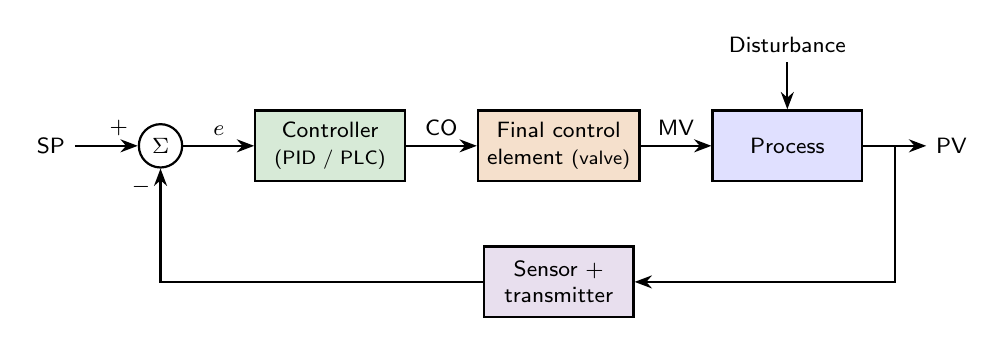
\begin{tikzpicture}[font=\footnotesize, node distance=0.9cm]
					\node[sumj] (s) {$\Sigma$};
					\node[left=0.8cm of s] (r) {SP};
					\node[blk, right=of s, fill=cGreen!18] (c) {Controller\\ \scriptsize(PID / PLC)};
					\node[blk, right=of c, fill=cOrange!20] (f) {Final control\\ element \scriptsize(valve)};
					\node[blk, right=of f, fill=blue!12] (p) {Process};
					\node[right=0.8cm of p] (y) {PV};
					\node[blk, below=0.8cm of f, fill=cPurple!15] (m) {Sensor +\\ transmitter};
					\node[above=0.6cm of p] (d) {Disturbance};
					\draw[sig] (r) -- node[above, pos=0.7] {$+$} (s);
					\draw[sig] (s) -- node[above] {$e$} (c);
					\draw[sig] (c) -- node[above] {CO} (f);
					\draw[sig] (f) -- node[above] {MV} (p);
					\draw[sig] (p) -- coordinate[pos=0.5] (tap) (y);
					\draw[sig] (d) -- (p);
					\draw[sig] (tap) |- (m);
					\draw[sig] (m) -| node[left, pos=0.92] {$-$} (s);
				\end{tikzpicture}
			\end{center}

			\textbf{(b) Elements}
			\begin{itemize}[itemsep=1pt]
				\item \textbf{Setpoint (SP)} --- the desired value of the controlled variable.
				\item \textbf{Summing junction / comparator} --- forms the error $e = \text{SP} - \text{PV}$.
				\item \textbf{Controller} --- decides the corrective output (CO) from the error (ON--OFF, PID, PLC logic).
				\item \textbf{Final control element} --- valve, pump or motor that changes the manipulated variable (MV).
				\item \textbf{Process (plant)} --- the equipment whose variable is controlled.
				\item \textbf{Sensor / transmitter} --- measures the process variable (PV) and sends a standard signal (4--20 mA).
				\item \textbf{Disturbance} --- any external change that upsets the PV (e.g.\ change in outflow).
			\end{itemize}

			\textbf{(c) Open loop vs.\ closed loop}
			\begin{center}
				\small
				\begin{tabular}{@{}p{3.2cm}p{5.4cm}p{5.4cm}@{}}
					\toprule
					\textbf{Feature} & \textbf{Open loop} & \textbf{Closed loop} \\
					\midrule
					Feedback     & none                    & output measured and fed back \\
					Accuracy     & depends on calibration  & high, self-correcting \\
					Disturbances & not corrected           & automatically corrected \\
					Stability    & always stable           & can oscillate if badly tuned \\
					Cost         & low                     & higher (sensor + controller) \\
					Example      & toaster timer           & thermostat, autopilot \\
					\bottomrule
				\end{tabular}
			\end{center}

			\textbf{(d) Example --- tank level control:} a level transmitter (LT) measures the water level and sends 4--20 mA to the level controller (LC). The LC compares it with the setpoint (say 1.5 m); if the level is low it opens the inlet control valve further, if high it closes it. If the outflow increases (disturbance), the level starts to fall, the error grows, and the controller opens the valve until the level returns to 1.5 m --- without any operator action.
		\end{answer}

		% -------------------------------------------------------------
		\item Explain the elements of a pneumatic system with a block diagram. Draw and explain the circuit of a double-acting cylinder controlled by a 5/2 single-solenoid valve. Calculate the extending and retracting forces of a cylinder of bore 50 mm and rod 20 mm at 6 bar. \qmarks{10}
		\begin{answer}
			\textbf{(a) Elements of a pneumatic system}
			\begin{center}
				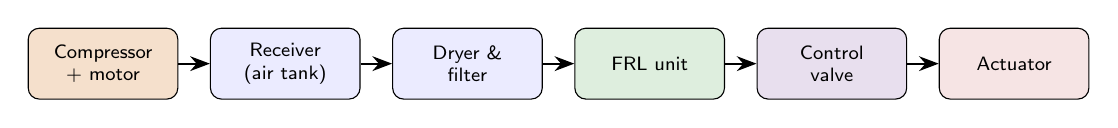
\begin{tikzpicture}[every node/.style={font=\scriptsize}, node distance=0.4cm,
					el/.style={rectangle, draw=black, rounded corners, minimum width=1.9cm, minimum height=0.9cm, align=center, fill=blue!8}]
					\node[el, fill=cOrange!20] (comp) {Compressor\\ + motor};
					\node[el, right=of comp] (rec) {Receiver\\ (air tank)};
					\node[el, right=of rec] (dry) {Dryer \&\\ filter};
					\node[el, right=of dry, fill=cGreen!15] (frl) {FRL unit};
					\node[el, right=of frl, fill=cPurple!15] (dcv) {Control\\ valve};
					\node[el, right=of dcv, fill=cRed!12] (act) {Actuator};
					\draw[flowarrow] (comp) -- (rec); \draw[flowarrow] (rec) -- (dry); \draw[flowarrow] (dry) -- (frl);
					\draw[flowarrow] (frl) -- (dcv); \draw[flowarrow] (dcv) -- (act);
				\end{tikzpicture}
			\end{center}
			\begin{itemize}[itemsep=1pt]
				\item \textbf{Compressor} raises atmospheric air to 6--10 bar; the \textbf{receiver} stores air and damps pulsations.
				\item \textbf{Dryer and filter} remove moisture and dirt that would corrode and jam valves.
				\item \textbf{FRL}: filter (fine cleaning), regulator (constant working pressure), lubricator (oil mist for moving parts).
				\item \textbf{Directional control valves} route the air; flow control valves set the speed.
				\item \textbf{Actuators} (cylinders, air motors) convert air pressure into motion.
			\end{itemize}

			\textbf{(b) Double-acting cylinder circuit}
			\begin{center}
				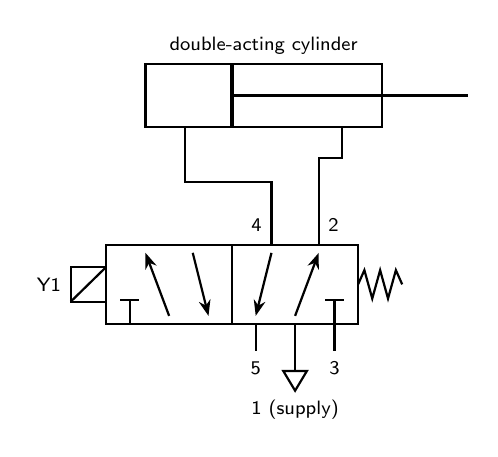
\begin{tikzpicture}[font=\scriptsize]
					\draw[thick] (0.5,2.5) rectangle (3.5,3.3);
					\draw[very thick] (1.6,2.5) -- (1.6,3.3);
					\draw[very thick] (1.6,2.9) -- (4.6,2.9);
					\node[above] at (2.0,3.3) {double-acting cylinder};
					\draw[thick] (0,0) rectangle (1.6,1);
					\draw[thick] (1.6,0) rectangle (3.2,1);
					\draw[vflow] (0.8,0.1) -- (0.5,0.9);
					\draw[vflow] (1.1,0.9) -- (1.3,0.1);
					\vblock{0.3}{0}{0.3}
					\draw[vflow] (2.4,0.1) -- (2.7,0.9);
					\draw[vflow] (2.1,0.9) -- (1.9,0.1);
					\vblock{2.9}{0}{0.3}
					\vsolenoid{0}{0.5}
					\node[left] at (-0.45,0.5) {Y1};
					\vspring{3.2}{0.5}
					\draw[thick] (1.9,0) -- (1.9,-0.35) node[below] {5};
					\draw[thick] (2.4,0) -- (2.4,-0.6);
					\draw[thick] (2.9,0) -- (2.9,-0.35) node[below] {3};
					\filldraw[fill=white, thick] (2.25,-0.6) -- (2.55,-0.6) -- (2.4,-0.85) -- cycle;
					\node[below] at (2.4,-0.85) {1 (supply)};
					\draw[thick] (2.1,1) -- (2.1,1.8) -- (1.0,1.8) -- (1.0,2.5);
					\draw[thick] (2.7,1) -- (2.7,2.1) -- (3.0,2.1) -- (3.0,2.5);
					\node[left] at (2.1,1.25) {4};
					\node[right] at (2.7,1.25) {2};
				\end{tikzpicture}
			\end{center}
			\begin{itemize}[itemsep=1pt]
				\item \textbf{Rest position} (spring side): port 1 $\rightarrow$ 2 supplies the rod side, port 4 $\rightarrow$ 5 exhausts the cap side $\Rightarrow$ the piston \textbf{retracts}.
				\item \textbf{Solenoid Y1 energised}: the valve shifts; 1 $\rightarrow$ 4 supplies the cap side, 2 $\rightarrow$ 3 exhausts $\Rightarrow$ the piston \textbf{extends}.
				\item De-energising Y1 lets the spring return the valve, and the cylinder retracts.
			\end{itemize}

			\textbf{(c) Force calculation} ($p = 6$ bar $= 0.6$ N/mm$^2$)
			\[
			A_{\text{cap}} = \tfrac{\pi}{4}(50)^2 = 1963\ \text{mm}^2 \Rightarrow F_{\text{ext}} = 0.6\times1963 \approx \mathbf{1178\ N}
			\]
			\[
			A_{\text{ann}} = \tfrac{\pi}{4}(50^2-20^2) = 1649\ \text{mm}^2 \Rightarrow F_{\text{ret}} = 0.6\times1649 \approx \mathbf{990\ N}
			\]
			The retracting force is smaller because the rod occupies part of the piston area.
		\end{answer}

		% -------------------------------------------------------------
		\item Draw the block diagram of a PID controller and explain the effect of the P, I and D actions. Describe the Ziegler--Nichols closed-loop tuning method with a flowchart, and find the PID settings for $K_u = 10$ and $P_u = 2$ s. \qmarks{10}
		\begin{answer}
			\textbf{(a) PID control law and block diagram}
			\[
			u(t) = K_p\,e(t) + K_i\!\int_0^t e\,d\tau + K_d\,\frac{de}{dt},
			\qquad K_i = \frac{K_p}{T_i},\; K_d = K_p T_d
			\]
			\begin{center}
				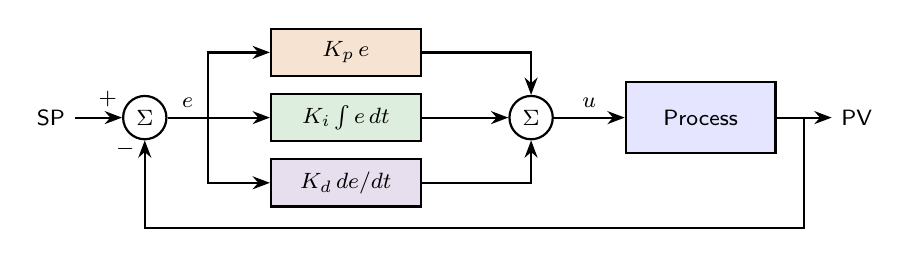
\begin{tikzpicture}[font=\footnotesize, node distance=0.9cm]
					\node (r) {SP};
					\node[sumj, right=0.6cm of r] (s1) {$\Sigma$};
					\node[blk, right=1.3cm of s1, fill=cGreen!15, minimum height=0.6cm] (i) {$K_i\int e\,dt$};
					\node[blk, above=0.2cm of i, fill=cOrange!18, minimum height=0.6cm] (p) {$K_p\,e$};
					\node[blk, below=0.2cm of i, fill=cPurple!15, minimum height=0.6cm] (d) {$K_d\,de/dt$};
					\node[sumj, right=1.1cm of i] (s2) {$\Sigma$};
					\node[blk, right=0.9cm of s2, fill=blue!10] (pl) {Process};
					\node[right=0.7cm of pl] (y) {PV};
					\draw[sig] (r) -- node[above, pos=0.7] {$+$} (s1);
					\draw[thick] (s1) -- node[above] {$e$} ++(0.8,0) coordinate (br);
					\draw[sig] (br) |- (p.west); \draw[sig] (br) -- (i.west); \draw[sig] (br) |- (d.west);
					\draw[sig] (p.east) -| (s2.north); \draw[sig] (i.east) -- (s2.west); \draw[sig] (d.east) -| (s2.south);
					\draw[sig] (s2) -- node[above] {$u$} (pl);
					\draw[sig] (pl) -- coordinate[pos=0.5] (tap) (y);
					\draw[sig] (tap) -- ++(0,-1.4) -| node[left, pos=0.95] {$-$} (s1.south);
				\end{tikzpicture}
			\end{center}

			\textbf{(b) Effect of each action}
			\begin{center}
				\small
				\begin{tabular}{@{}lcccc@{}}
					\toprule
					\textbf{Increase} & \textbf{Rise time} & \textbf{Overshoot} & \textbf{Settling time} & \textbf{Steady-state error} \\
					\midrule
					$K_p$ & decreases & increases & small change & decreases \\
					$K_i$ & decreases & increases & increases & \textbf{eliminated} \\
					$K_d$ & small change & decreases & decreases & no effect \\
					\bottomrule
				\end{tabular}
			\end{center}
			\textbf{P} gives a fast response proportional to the present error but leaves an offset; \textbf{I} acts on the accumulated past error and removes the offset; \textbf{D} acts on the rate of change (predicts the future error), adds damping, but amplifies noise.

			\textbf{(c) Ziegler--Nichols closed-loop method --- flowchart and settings}

			\noindent\begin{minipage}[c]{0.58\linewidth}\centering
			
				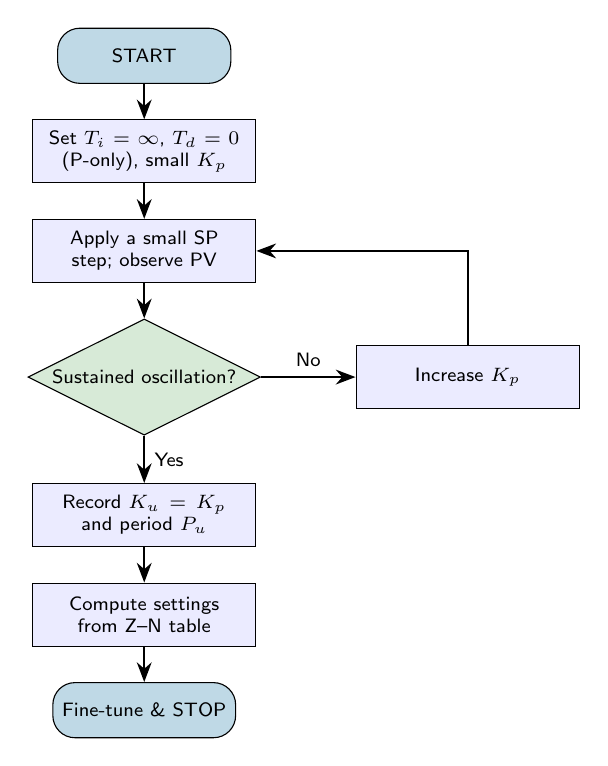
\begin{tikzpicture}[font=\scriptsize, node distance=0.45cm]
					\node[startstop] (st) {START};
					\node[process, below=of st] (a) {Set $T_i = \infty$, $T_d = 0$ (P-only), small $K_p$};
					\node[process, below=of a] (b) {Apply a small SP step; observe PV};
					\node[decision, below=of b] (c) {Sustained oscillation?};
					\node[process, right=1.2cm of c] (inc) {Increase $K_p$};
					\node[process, below=0.6cm of c] (rec) {Record $K_u = K_p$ and period $P_u$};
					\node[process, below=of rec] (tab) {Compute settings from Z--N table};
					\node[startstop, below=of tab] (en) {Fine-tune \& STOP};
					\draw[flowarrow] (st) -- (a); \draw[flowarrow] (a) -- (b); \draw[flowarrow] (b) -- (c);
					\draw[flowarrow] (c) -- node[above] {No} (inc);
					\draw[flowarrow] (inc) |- (b);
					\draw[flowarrow] (c) -- node[right] {Yes} (rec);
					\draw[flowarrow] (rec) -- (tab); \draw[flowarrow] (tab) -- (en);
				\end{tikzpicture}
			
			\end{minipage}\hfill
			\begin{minipage}[c]{0.40\linewidth}\centering
			
				\small
				\begin{tabular}{@{}lccc@{}}
					\toprule
					\textbf{Controller} & $K_p$ & $T_i$ & $T_d$ \\
					\midrule
					P   & $0.5K_u$  & $\infty$  & 0 \\
					PI  & $0.45K_u$ & $P_u/1.2$ & 0 \\
					PID & $0.6K_u$  & $P_u/2$   & $P_u/8$ \\
					\bottomrule
				\end{tabular}
			
				\par\medskip\footnotesize $K_u$ = ultimate gain, $P_u$ = period of the sustained oscillation.
			\end{minipage}

			\medskip
			\textbf{(d) Numerical} ($K_u = 10$, $P_u = 2$ s):
			\[
			K_p = 0.6\times10 = \mathbf{6},\quad T_i = 2/2 = \mathbf{1\ s},\quad T_d = 2/8 = \mathbf{0.25\ s}
			\]
			\[
			K_i = K_p/T_i = 6\ \text{s}^{-1},\qquad K_d = K_pT_d = 1.5\ \text{s}
			\]
			These values give a fast response with about 25\,\% overshoot and are used as a starting point for fine-tuning.
		\end{answer}

	\end{enumerate}

\end{document}
